\section{Deep Learning}

In this section I am referencing information from the book \textit{Deep Learning} \cite{Goodfellow-et-al-2016} chapters 1 and 10.
\\
Computers are good in solving problems which can be described formally by mathematical rules. There are problems easy for humans but hard to be formally described.  With lots of training data system can gather knowledge from experience without the need for human to specify all needed concepts. System is building a hierarchical graph of concepts which enables him to learn complicated concepts from similar ones. Cause this graph of concepts is very deep we call this approach \textbf{Deep Learning}.

\subsection{Recurrent neural network}

Recurrent neural networks (RRNs) are family of neural networks specialized for processing sequential data. RNNs are made to process sequences of values $ x^{(1)}, x^{(2)},x^{(3)}, ..., x^{(n)} $. They can process long sequences and most of recurrent networks can work also with sequences with variable length. 

For processing sequences of fixed length we can use simple multi-layer perceptron model, however this model is not able to efficiently learn  dependencies between inputs. For example in language word order might not change the meaning of sentence. 
\begin{center}
    \textbf{In last year, there were Covid pandemic.}\\
    \textbf{There were Covid pandemic last year.}
\end{center}
Meaning of both sequences is the same but the target words \textit{Covid pandemic} are not in the same place in these sentences. We want from network to accumulate knowledge from previous input words in processing of next word. In RNNs same function of previous output and current input is used for each input. This process stores information from previous time point in so called \textbf{hidden state} $h^{(t)}$. We can better imagine this process by unfolding neural network in time.

\begin{figure}[!h]
    \centering
    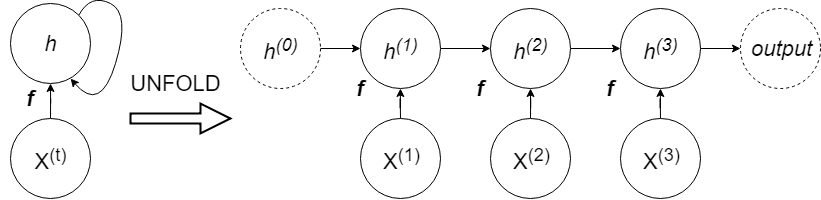
\includegraphics[width=140mm]{chapters/images/RNN_unfold.png}
    \caption{Recurrent neural network processing information of length 3}
    \label{fig:Unfold}
\end{figure}

Each node in unfolded graph represents one time instance. We can rewrite one step computation
$$ h^{(t)} = f(h^{(t-1)}, x^{(t-1)}, \Theta)$$

It is proven that any function computable by a Turing machine can be computed by RNN of a finite size.

\subsubsection{Leaky recurrent neural network}

Problem with big RNN is vanishing or exploding gradient. Unfolded graph of RNN acts like multi-layer perceptron. If sequences are long our imaginary network is very deep. In backward pass is likely that gradient will vanish to have absolutely zero effect on previous inputs, or explode and focus only on one example. Leaky RNNs have lateral connections in time to avoid this effect (figure \ref{fig:RNN_lateral}). They accumulate information over long time.  

\begin{figure}[!h]
    \centering
    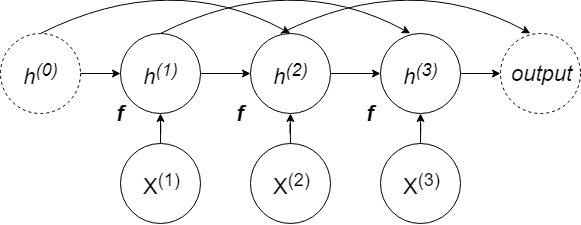
\includegraphics[width=140mm]{chapters/images/RNN_leaky.png}
    \caption{Recurrent neural network with lateral connections every second time instance }
    \label{fig:RNN_lateral}
\end{figure}

\subsection{Long short term memory - LSTM}

Leaky RNN accumulate information over long period of time. However in some cases we want to forget part of information we learned, for example if our sequence consists of subsequences. This problem was solved by introducing gated units like \textbf{LSTM}. Gated unit use gates - learnable parameters which controls amount of information passing through. 


\begin{figure}[!h]
    \centering
    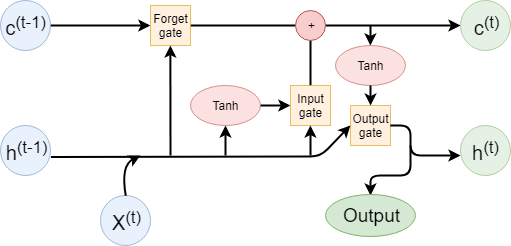
\includegraphics[width=140mm]{chapters/images/LSTM.png}
    \caption{LSTM unit}
    \label{fig:LSTM}
\end{figure}

LSTM has three two states. 
\begin{itemize}
    \item $c^{(t)}$ represents \textbf{cell state} - cell state is a path for information to run down through whole network like lateral connections in leaky units
    \item $h^{(t)}$ represents \textbf{hidden state} - hidden state is previous output of LSTM.
\end{itemize}

LSTM also have three gates: Input, output and forget gate. Each gate is a pointwise multiplication of first input and output of nonlinear function from second input (fig. \ref{fig:LSTM_gate}). Gate has two weight matrices $U$ for input vector and $W$ for hidden state vector.


\begin{figure}[!h]
    \centering
    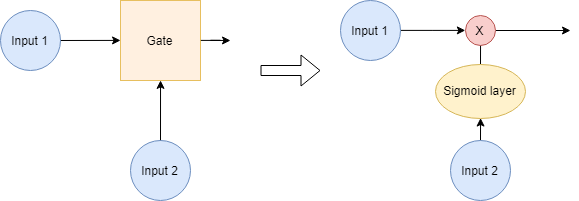
\includegraphics[width=120mm]{chapters/images/LSTM_gate.png}
    \caption{Gate}
    \label{fig:LSTM_gate}
\end{figure}

Input $x^{(t)}$ is at first concatenated with hidden state $h^{(t-1)}$ and with $c^{(t-1)}$ goes through Forget gate. Let $f^{(t)}$ be the output from sigmoid layer from the gate.

\begin{eqnarray}
    f^{(t)} = \sigma \left(  bias^f + \sum_j U^f_{i,j} x^{(t)}_j + \sum_j W^f_{i,j} h^{(t-1)}_j \right)
\end{eqnarray}

Next cell state is then computed:


\begin{eqnarray}
    I^{(t)} = \sigma \left(  bias^I + \sum_j U^I_{i,j} x^{(t)}_j + \sum_j W^I_{i,j} h^{(t-1)}_j \right) \\
    l^{(t)} = tanh \left(  bias^l + \sum_j U^l_{i,j} x^{(t)}_j + \sum_j W^l_{i,j} h^{(t-1)}_j \right) \\
    c^{(t)} = f^{(t)}c^{(t-1)} + I^{(t)}l^{(t)}
\end{eqnarray}

where $I^{(t)}l^{(t)}$ is output of input gate and $l^{(t)}$ is LSTM internal unit.

Next hidden state is computed 
\begin{eqnarray}
    O^{(t)} = \sigma \left(  bias^O + \sum_j U^O_{i,j} x^{(t)}_j + \sum_j W^O_{i,j} h^{(t-1)}_j \right) \\
    h^{(t)} = tanh(c^{(t)}) O^{(t)}
\end{eqnarray}

Let $n$ be the size of input vector and $m$ size of hidden state vector. At the end LSTM unit consists of four pairs of matrices - $W$ with shape $m \times m$ and $U$ with shape $m \times n$. Total number of trainable parameters is then 
\begin{equation}
N = 4 \cdot ( n \times m ) 
\end{equation}

LSTM network have been shown to learn long-term dependencies more easily than the simpler recurrent neural networks. LSTM are good for forecasting time series. Input for the system is some subsequence of time series and output is next point in time series.  

One disadvantage of LSTM is length of training. Using time folding with this many parameters cause long training of LSTM even with relatively low input and hidden dimensions.

\section{PyTorch}

Pytorch is an open source machine learning framework developed by Facebook \cite{PytotchDocumentation}. In this section I am referencing resources \cite{Pytorch} and \cite{PytotchDocumentation}. 

Pytorch is Python framework which allows to write model in easy to read idiomatic Python. Due easy debugging and clear syntax, Pytorch has been used by research communities and is very good as introduction to deep learning. Pytorch provide accelerated computations using GPUs, which can be $50 \times$ faster than same operations computer on CPU.

\subsection{Autograd}

Autograd is component in Pytorch which is responsible for automatic computation of gradient. PyTorch \textit{tensor} is able to remember all operations performed on him. Autograd can computer derivatives of this operations with respect to their inputs. 

This is essential for computing gradients in backpropagation algorithm in deep neural networks where analytic solutions for gradients are very complex.

\begin{lstlisting}[language=Python]
>>> import torch
>>> x = torch.tensor([5.], requires_grad=True)
>>> z = x**2
>>> z
tensor([25.], grad_fn=<PowBackward0>)
>>> x.grad
None
>>> z.backward()  # calling of autograd
>>> x.grad
tensor([10.])
\end{lstlisting}

As we can see in code example we are computing derivative of function $f(x) = x^2$ with respect to $x$. We can confirm that derivative $\frac{d x^2}{d x} = 10$

$$ \frac{d x^2}{d x} = 2x = 2\cdot 5 = 10 $$

Every \textit{tensor} has \textit{grad} attribute which is filled after call of autograd. If option \textit{requires\_grad} is set to \textit{True} gradients are computes with respect to this variable.

\subsection{Neural network model}

In Pytorch we define neural network model as Python class derived from \textit{nn.Model} class. Class must implement these methods
\begin{enumerate}
    \item \textbf{\_\_init\_\_} - in this function we define our layers
    \item \textbf{forward} - this function implement forward pass of our network.
\end{enumerate}

\begin{lstlisting}[language=Python]
class SimpleNet(nn.Module):
    def __init__(self):
        super(SimpleNet, self).__init__()
        self.l1 = nn.Linear(10,2)
    
    def forward(self, x):
        y = self.l1(x)
        return torch.tanh(y)
\end{lstlisting}


This is all we need for our simple network. Backpropagation in the training is made by Optimizer from package \textit{torch.optim}.
